
\section{Methodology}
We are aiming to improve RTE by leveraging the collaboratively collected real-world interactions.
To be clear about the terminology, in repertoire-based method, an interaction means executing an certain elementary policy and acquiring its outcome.
DP enables us to achieve this by extending the GP model in RTE to an infinite mixture of GPs trained with real-world data.
Previous works of training infinite mixture of GP via DP have been made in \cite{infinite_MGP, variational_MGP}. 
But in our case, the design needs to be different.
First, our real-world interaction data are produced in individual episodes, where each episode corresponds to the interactions collected during each deployment.
Since we know that each deployment is made in a certain environment, all the interactions in an episode should correspond to the same dynamics. 
Hence, when clustering the historical data we need to conduct clustering on the episode but not on the individual data. 
The second difference from previous works is that we are decoupling each dimension and each episode.
The decoupling of dimension is inherited from RTE, while the decoupling of episodes is a unique design.
This is based on the fact that data within each episode come from the same environment and are hence correlated, while different episodes do not necessarily correspond to the same environment even they are grouped into the same cluster.
Such design allows us to group up environments that are different but similar, providing higher flexibility.
Another reason for using decoupled episodes is to make our system scalable.
Since we are now clustering episodes which typically contains dozens of data, each clusters can have thousands of data.
GP requires to compute the inverse of the joint covariance matrix, which has time complexity scaling cubic with data size.
Such computational expense is completely unaffordable for online adaptation. 
If the episodes are decoupled, the joint covariance matrix becomes a block diagonal matrix, and the time complexity of its inverse scales only linearly.




To really implement the DP clustering, there are many remaining challenges to be addressed.
The prior mean and kernel are the two most important factors of a GP.
It can be very hard to design a good prior function or to determine the length scales as we have little knowledge about the real-world dynamics.
A few parts of our methodology heavily rely on simulation.
For this, the simulation has to be relatively accurate and free of bugs.
We also make a very strong assumption that the simulated results always correspond to real-world outcomes in some environment. 
For example, we set the friction coefficient to 0.9 in the simulation, but the friction is underestimated and the simulated outcomes are very close to the real-world results for friction coefficient equal to 0.8.
Hence we believe that although the simulated results are not strictly accurate, they can still represent some real-world results.
This assumption not always true, but it plays a very important role in the methodology.



\subsection{Linear Prior Mean Function}
In GP, the prior mean function gives a prior estimate of the outcomes of all the elementary policies in a certain environment.
To study the dynamics, we express its dependency in the following form:
\begin{equation}
x_d(\bm{\beta}, \bm{\epsilon}) = f_d(\bm{\beta}, \bm{\epsilon}) 
+ g_d(\bm{\beta}) 
+ h_d(\bm{\epsilon}) + c_d 
\label{dynamics_assumption}
\end{equation}
where the $x_d$ stands for the $d^{\text{th}}$ dimension of the policy outcome (for example, this can be the robot displacement in the $x$ axis). Vector $\bm{\beta}$ represents the behaviour descriptor of the controller; vector $\bm{\epsilon}$ is the environment descriptor, representing some quantities of the environment. 
It can be seen from Eq. (\ref{dynamics_assumption}) that the dynamics consists of a term that depends on both the policy behaviour and the environment plus the terms that only depends on either the behaviour or environment plus a constant $c_d$.
Note that we do not require access to the $\bm{\beta}$ and $\bm{\epsilon}$ or knowing their detailed meanings.
Eq. (\ref{dynamics_assumption}) is generally non-linear. But in the case where the dynamics is relatively simple, like the use of periodic controller in RTE, we can get an approximation of it by Taylor expanding the $f_d(\bm{\beta}, \bm{\epsilon})$ term to the second order:
\begin{equation}
\begin{gathered}
f_d(\bm{\beta}, \bm{\epsilon}) \approx
f_d(\bm{\beta}_0, \bm{\epsilon}_0) + 
\begin{bmatrix}
J_{\bm{0, \beta}} & J_{\bm{0, \epsilon}} \\
\end{bmatrix}
%
\begin{bmatrix}
\Delta \bm{\beta} \\
\Delta \bm{\epsilon}
\end{bmatrix}
%
\\
%
+ \frac{1}{2}
\begin{bmatrix}
\Delta \bm{\beta}^T & \Delta \bm{\epsilon}^T \\
\end{bmatrix}
%
\begin{bmatrix}
H_{\bm{0, \beta \beta}} & H_{\bm{0}, \bm{\beta \epsilon}} \\
H_{\bm{0, \epsilon \beta}} & H_{\bm{0, \epsilon \epsilon}} \\
\end{bmatrix}
%
\begin{bmatrix}
\Delta \bm{\beta} \\
\Delta \bm{\epsilon}
\end{bmatrix}
\end{gathered}
\label{Taylor_expansion}
\end{equation}
where the Jacobian vector $J_{\bm{0}}$ and the Hessian matrix $H_{\bm{0}}$ have been arranged in the partitioned form, and their subscript 0 denotes they are evaluated at $(\bm{\beta}_0, \bm{\epsilon}_0)$.
We then substitute this result into Eq. (\ref{dynamics_assumption}) to arrive at:
\begin{equation}
\begin{gathered}
x_d(\bm{\beta}, \bm{\epsilon}) \approx
\Delta \bm{\beta}^T H_{\bm{0, \beta \epsilon}} \Delta \bm{\epsilon}
+ f_d(\bm{\beta}_0, \bm{\epsilon}_0) + c_d
\\ + 
\frac{1}{2} \Delta \bm{\beta}^T H_{\bm{0, \beta \beta}} \Delta \bm{\beta} 
+ J_{\bm{0, \beta}} \Delta \bm{\beta}
+ g_d(\bm{\beta}) 
\\
+ \frac{1}{2} \Delta \bm{\epsilon}^T H_{\bm{0, \epsilon \epsilon}} \Delta \bm{\epsilon}
+ J_{\bm{0, \epsilon}} \Delta \bm{\epsilon}
+ h_d(\bm{\epsilon}) 
\end{gathered}
\label{approximation}
\end{equation}
%
Comparing Eq. (\ref{approximation}) with Eq. (\ref{dynamics_assumption}), we can see our approximation factorizes the correlated term. If the same policy is executed in two different environment, the difference in the dynamics will be:
\begin{equation}
\begin{gathered}
x_d(\bm{\beta}, \bm{\epsilon}_1) - 
x_d(\bm{\beta}, \bm{\epsilon}_2) \approx
\Delta \bm{\beta}^T H_{\bm{0, \beta \epsilon}} 
(\bm{\epsilon}_1 - \bm{\epsilon}_2)
\\
+ h^*_d(\bm{\epsilon}_1) - h^*_d(\bm{\epsilon}_2) 
\\
\text{where \,}
h^*_d(\bm{\epsilon}) = 
\frac{1}{2} \Delta \bm{\epsilon}^T H_{\bm{0, \epsilon \epsilon}} \Delta \bm{\epsilon}
+ J_{\bm{0, \epsilon}} \Delta \bm{\epsilon}
+ h_d(\bm{\epsilon}) 
\end{gathered}
\label{dynamics_diff}
\end{equation}
If we treat the $h^*_d(\bm{\epsilon})$ term as an additional dimension of the environment vector, then Eq. (\ref{dynamics_diff}) can be represented as:
\begin{equation}
\begin{gathered}
\Delta \bm{x}_d = 
\begin{bmatrix}
\Delta x_{d, 1} \\
\vdots \\
\Delta x_{d, N} \\
\end{bmatrix}
\approx
\begin{bmatrix}
\Delta \bm{\beta}_1^T H_{\bm{0, \beta \epsilon}} & 1 \\
\vdots & \vdots \\
\Delta \bm{\beta}_N^T H_{\bm{0, \beta \epsilon}} & 1 \\
\end{bmatrix}
\Delta \bm{\varepsilon} 
\\
= W_{d}^T \Delta \bm{\varepsilon}
\end{gathered}
\label{linear_form}
\end{equation}
where $\bm{\varepsilon}$ is our new environment vector. 
The vector $\Delta \bm{x}_d$ stands for the difference in dynamics for the entire repertoire with each entry $\Delta x_{d, i}$ denoting the result for the each elementary policy.
Combined with the assumption we made about the simulation, Eq. (\ref{linear_form}) suggests we may approximate the real-world distortion of the entire repertoire using a linear model. 


The above derivations can be extended to any order of Taylor expansion, but the dimension of the new environment vector $\bm{\varepsilon}$ increases exponentially after the second order.
If we assume the dynamics can be efficiently approximated with the second order expansion, Eq. (\ref{linear_form}) gives a very potent result.
However, we do not have access to the matrix $W_d$ or the environment vector $\bm{\varepsilon}$ directly. 
Instead, we can leverage the fact that any environment vector can be linearly represented by a set of environment vectors as the basis.
Hence, if we have collected enough distortions, any new distortion can be  represented with a linear combination of the collected ones:
\begin{equation}
\begin{gathered}
\Delta \bm{x}_d^* \approx
W_{d}^T \Delta \bm{\varepsilon}^* = 
W_{d}^T
\begin{bmatrix}
\Delta \bm{\varepsilon}^{(1)}, \cdots, \Delta \bm{\varepsilon}^{(n)}
\end{bmatrix}
\begin{bmatrix}
\omega_1^* \\
\vdots \\
\omega_n^* \\
\end{bmatrix}
\\ =
\begin{bmatrix}
\Delta \bm{x}_d^{(1)}, \cdots, \Delta \bm{x}_d^{(n)}
\end{bmatrix}
\begin{bmatrix}
\omega_1^* \\
\vdots \\
\omega_n^* \\
\end{bmatrix}
\end{gathered}
\label{linear_combination}
\end{equation}
This means we need to get the distortions of all the elementary policies in several environments.
Since typically a repertoire can contain of a few thousand policies,
we cannot afford to do such amount of evaluations in the real-world, and hence we need to rely on simulation.


A question is that how many distortions we should collect.
If we get too few distortions, we might not have collected all the basis, and the linear model will perform poorly in uncovered environments.
On the other hand, if we have collected too many, not only will this be computationally expensive but this will also lead to very large dimensions. 
The solution is collect as many as we can afford and then reduce the dimensionality with singular vector decomposition (SVD). The collection of distortions can be represented as:
\begin{equation}
\bm{A} = 
\begin{bmatrix}
\Delta \bm{x}_d^{(1)}, \cdots, \Delta \bm{x}_d^{(n)}
\end{bmatrix}
= \sum_{i=1}^s \sigma_i \bm{v}_i \bm{u}_i^T
\label{SVD}
\end{equation}
where $\bm{v}_i$ stands for each normalized base vector and $\bm{u}_i$ is the normalized component of this base vector in each distortion.
The number of basis $s$ is much smaller than $n$ as we have collected more than we need to ensure a good coverage.
To conduct SVD, we left multiply matrix $\bm{A}$ by its transpose:
\begin{equation}
\begin{gathered}
\bm{A}^T \bm{A} = 
\sum_{i=1}^s \sigma_i^2 \bm{u}_i \bm{u}_i^T = \bm{U} \bm{D} \bm{U}^T
\\
\text{where \,}
\bm{U} = 
\begin{bmatrix}
\bm{u}_1, \cdots, \bm{u}_s
\end{bmatrix}
\text{, \,}
\bm{D} = 
\begin{bmatrix}
\sigma_1^2 &  &  \\
 & \ddots &  \\
 &  & \sigma_s^2 \\
\end{bmatrix}
\end{gathered}
\label{ATA}
\end{equation}
According to spectral theorem, entry $\sigma^2$ and vectors $\bm{u}$  are the non-zero eigenvalues and the corresponding eigenvectors of $\bm{A}^T\bm{A}$, respectively. 
The desired base vectors can then be calculated:
\begin{equation}
\begin{gathered}
%\frac{1}{\sigma_j}\bm{A} \bm{u}_j = 
%\sum_{i=1}^s \frac{\sigma_i}{\sigma_j} \bm{v}_i \delta_{i,j}
%= \bm{v}_j
%\\
%\text{hence \,}
\begin{bmatrix}
\bm{v}_1, \cdots, \bm{v}_s
\end{bmatrix} = 
\sqrt{\bm{D}^{-1}} \bm{A} \bm{U}
\end{gathered}
\label{basis}
\end{equation}
The eigenvalues denote the importance of each base vector.
If an eigenvalue is zero, we can completely ignore this dimension as it can be linearly represented by other basis.
In practice, since evaluations are noisy and our linear relation is approximated, we will never get any zero eigenvalues. 
To continue with our dimensionality reduction, we can rearrange the eigenvalues in a descending order and keep only the first few terms depending on how many dimensions we wish to have.
Thus, we can approximate any real-world distortion using a linear combination of simulated distortions filtered by SVD.



\subsection{Determine the Input Space}
In GP, the prior mean function only provides an estimate of the dynamics, and the residual is modelled with probabilistic inference.
This requires the definition of input space for the kernel to build the covariance between observations.
In the RTE, the input space the same as the $x$ and $y$ displacements.
Considering the policies are generated using the MAP-Elites instead of gradient based methods, policies having similar displacements might have very different behaviours.
As a result, they may lead to very different outcomes in new environments, and the use of such input space could be misleading.
Hence, we aim to find the input space in which the distances between policies are related to their outcomes in all environments. 

By examining our assumption of dynamics in Eq. (\ref{linear_form}), we see that the behaviour vectors that are encoded in the $W_d$ matrix.
By rearranging Eq. (\ref{linear_form}), we can get:
\begin{equation}
\begin{gathered}
W_{d}^T \Delta \bm{\varepsilon} = 
\begin{bmatrix}
\Delta \bm{\beta}_1^T & 1\\
\vdots & \vdots \\
\Delta \bm{\beta}_N^T & 1\\
\end{bmatrix}
%
\begin{bmatrix}
H_{\bm{0, \beta \epsilon}} & 0 \\
\\
0 & 1 \\
\end{bmatrix}
\Delta \bm{\varepsilon}
\end{gathered}
\label{linear_form_for_beta}
\end{equation}
Since we have found the basis that can linearly represent any environment vector $\bm{\varepsilon}$, we can always find a particular set of $\bm{\varepsilon}$ such that:
\begin{equation}
\begin{gathered}
W_{d}^T
\begin{bmatrix}
\Delta \bm{\varepsilon}_1, \cdots , \Delta \bm{\varepsilon}_N
\end{bmatrix}
= \\
\begin{bmatrix}
\Delta \bm{\beta}_1^T & 1\\
\vdots & \vdots \\
\Delta \bm{\beta}_N^T & 1\\
\end{bmatrix}
%
\begin{bmatrix}
H_{\bm{0, \beta \epsilon}} & 0 \\
\\
0 & 1 \\
\end{bmatrix}
\begin{bmatrix}
H_{\bm{0, \beta \epsilon}}^T
(H_{\bm{0, \beta \epsilon}}H_{\bm{0, \beta \epsilon}}^T)^{-1} \\
\\
0 \\
\end{bmatrix}
\\ 
= 
\begin{bmatrix}
\Delta \bm{\beta}_1^T & 1\\
\vdots & \vdots \\
\Delta \bm{\beta}_N^T & 1\\
\end{bmatrix}
%
\begin{bmatrix}
\mathbf{I} \\
\\
0 \\
\end{bmatrix} 
= 
\begin{bmatrix}
\Delta \bm{\beta}_1^T \\
\vdots \\
\Delta \bm{\beta}_N^T \\
\end{bmatrix}
\end{gathered}
\label{beta}
\end{equation}
This means we are able to represent the behaviour vectors as a linear combination of the distortion basis we found for the linear prior mean function.
This is a very reasonable result since if two policies have similar outcomes across many environments, they are more likely to share similar distortions in a new environment.
Note that the above derivations only hold if the dimension of the behaviour vector is not larger than the dimension of environment vector, otherwise the $H_{\bm{0, \beta \epsilon}}H_{\bm{0, \beta \epsilon}}^T$ matrix is not invertible.
However, our purpose of finding the behaviour vectors is just to build statistical inference between policies, which tolerates uncertainties.
In the case there are omitted dimensions, we can just add a larger noise to the diagonal of the covariance matrix to incorporate this missing information.


It is hard to determine the detailed linear combination to get the behaviour vectors.
But considering the use of anisotropic length scales for the distance metric in Eq. (\ref{distance_metric}), it is desirable to find a linear combination to reduce the correlations between the dimensions.
This is achieved using principle component analysis (PCA) \cite{PCA}. We first find the empirical covariance matrix of the standardized distortions.
\begin{equation}
\begin{gathered}
\bm{\Sigma} = \bm{X}^T \bm{X}
\end{gathered}
\label{cov}
\end{equation}
$\bm{X}$ is a $N \times s$ matrix, where $N$ is the size of the repertoire (the amount of elementary policies) and $s$ is the number of basis found using SVD.
Each column of $\bm{X}$, namely each dimension of basis, is standardized across the policies.
The covariance matrix $\bm{\Sigma}$ is a real-symmetric matrix, according to spectral theorem, it can be represented by:
\begin{equation}
\begin{gathered}
\bm{\Sigma} = 
\sum_{i=1}^s \lambda_i \bm{u}_i \bm{u}_i^T = \bm{U} \bm{D} \bm{U}^T
\end{gathered}
\label{PCA}
\end{equation}
Similar to SVD, the $\lambda_i$ are the eigenvalues of the covariance matrix, and $\bm{U}$ contains the corresponding eigenvectors.
%Similar to SVD, these eigenvalues are non-negative and give the importance of each dimension (see Fig. \ref{}).
We can then find our input space with the following transform:
\begin{equation}
\begin{gathered}
\begin{bmatrix}
\bm{v}'_1, \cdots, \bm{v}'_s
\end{bmatrix}
=
\begin{bmatrix}
\bm{v}_1, \cdots, \bm{v}_s
\end{bmatrix}
\bm{U} \sqrt{\bm{D}^{-1}}
\end{gathered}
\label{input_space}
\end{equation}
This gives the coordinates of each elementary policy in our input space. Each dimension of the coordinates are now decorrelated (see Fig. \ref{PCA_outcome}).
Since this coordinate system is just a linear transformation of the SVD basis with full rank, it can also be used as the basis for the prior mean function.
Hence, we replace the previous basis by this coordinate system for simplicity, and the distortion estimated by the prior mean function becomes: 
\begin{equation}
\begin{gathered}
\Delta \bm{x}_{d} = 
\bm{X}_{d}
\bm{w}_{\varepsilon, d}
\end{gathered}
\label{prior_mean_function}
\end{equation}
where each row of $\bm{X}_{d}$ is the coordinates (for the $d^{\text{th}}$ dimension of dynamics) of the corresponding policy.
%
\begin{figure}[h]
\centering
\subfloat[]{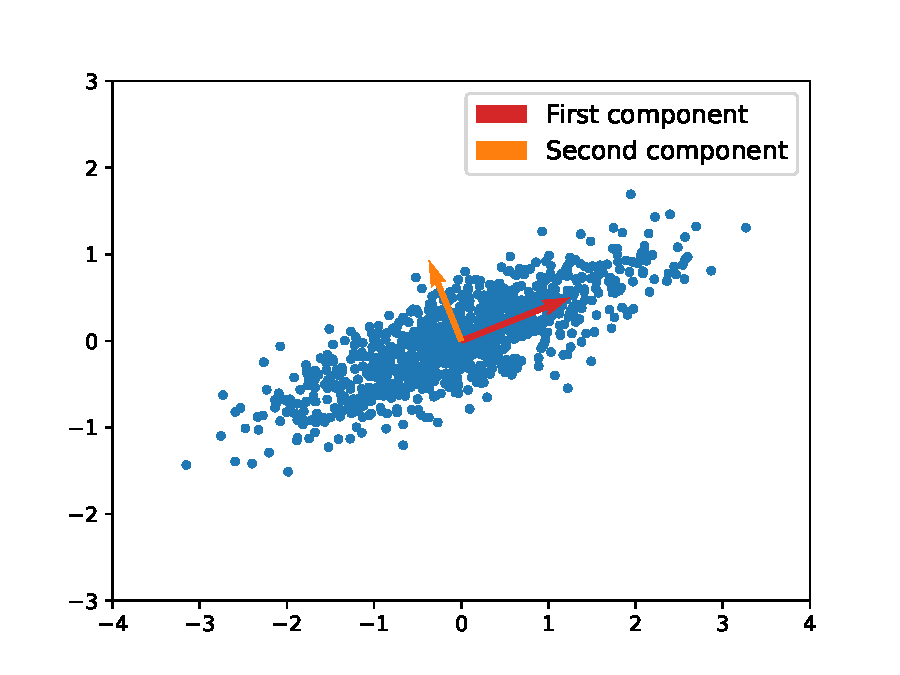
\includegraphics[width=0.255\textwidth]{before_pca.pdf}%
\label{fig_first_case}}
%\hfil
\subfloat[]{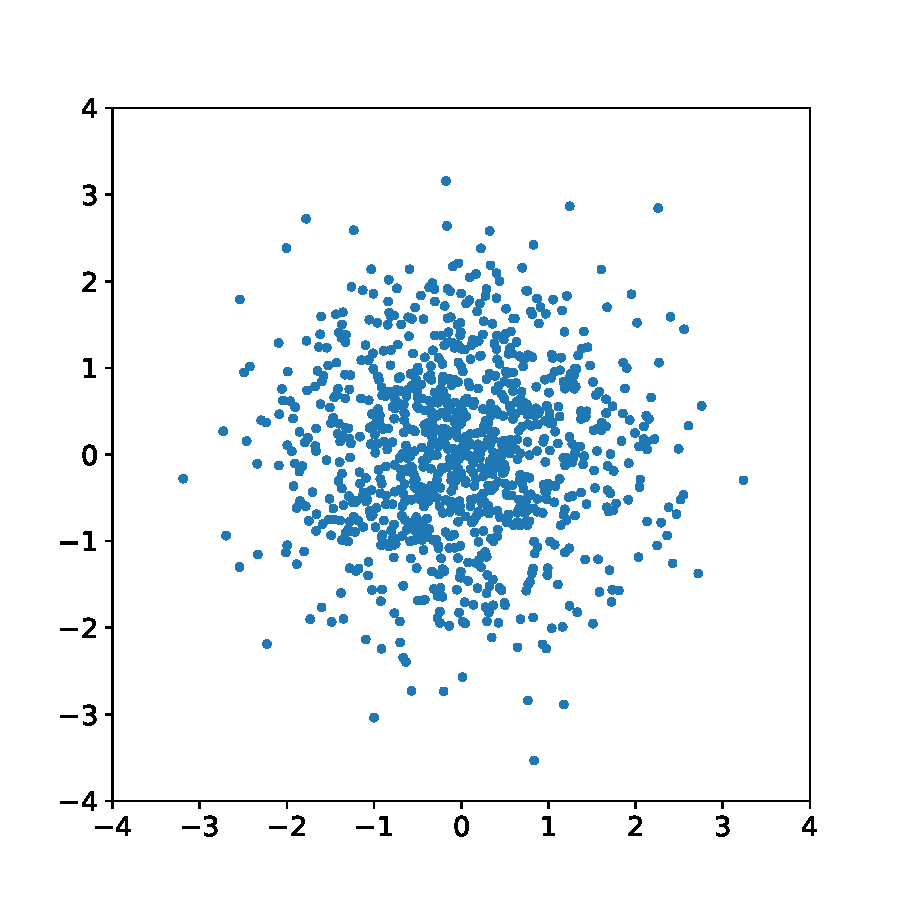
\includegraphics[width=0.195\textwidth]{after_pca.pdf}%
\label{fig_second_case}}
\caption{Example of PCA transform. Original data distribution is given by (a), where the two axes are highly correlated. (b) is the resultant distribution after applying Eq. (\ref{input_space}), where the correlation is removed.}
\label{PCA_outcome}
\end{figure}



\subsection{Choosing the Dynamics Representation}
We can use different representations of the dynamics $x_d$ in Eq. (\ref{dynamics_assumption}).
Apart from using $x$ and $y$ displacements (called displacement-based representation in this paper) as in RTE, another type of representation is investigated.
Since RTE uses periodic controllers, the robot will experience the same displacement and rotation during each period, and the execution should result in an arc.
Based on this analysis, we represent the dynamics as the tangential speed $v$, angular velocity $\omega$ and direction $\varphi$ (see Fig. \ref{arcs}). 
This design, called arc-based representation, considers the fact that the different dimensions of the dynamics are modelled by different GPs (hence are decoupled) in RTE.
This is not an ideal design since $x$ and $y$ are typically correlated.
In arc-based representation, these parameters are more decoupled and more consistent with real-world mechanics. 
Take a hexapod robot for example.
If the robot is carrying heavy payload and becomes slower, arc-based representation can easily model this distortion by reducing $v$ for all policies. However, for displacement-based representation, reduced speed will lead to decrease for positive displacements and increase for negative displacements.
In the case where the robot suffers damage in one of its legs, the side of the damaged leg will contribute lesser force, and the robot might move towards a different direction or rotate during the motion.
For arc-based representation, this can be modelled by adding a shift to the angular velocities and directions of the policies.
While it is a lot harder for the displacement-base representation, and $x$ and $y$ will become strongly correlated.
\begin{figure}[h]
\centering
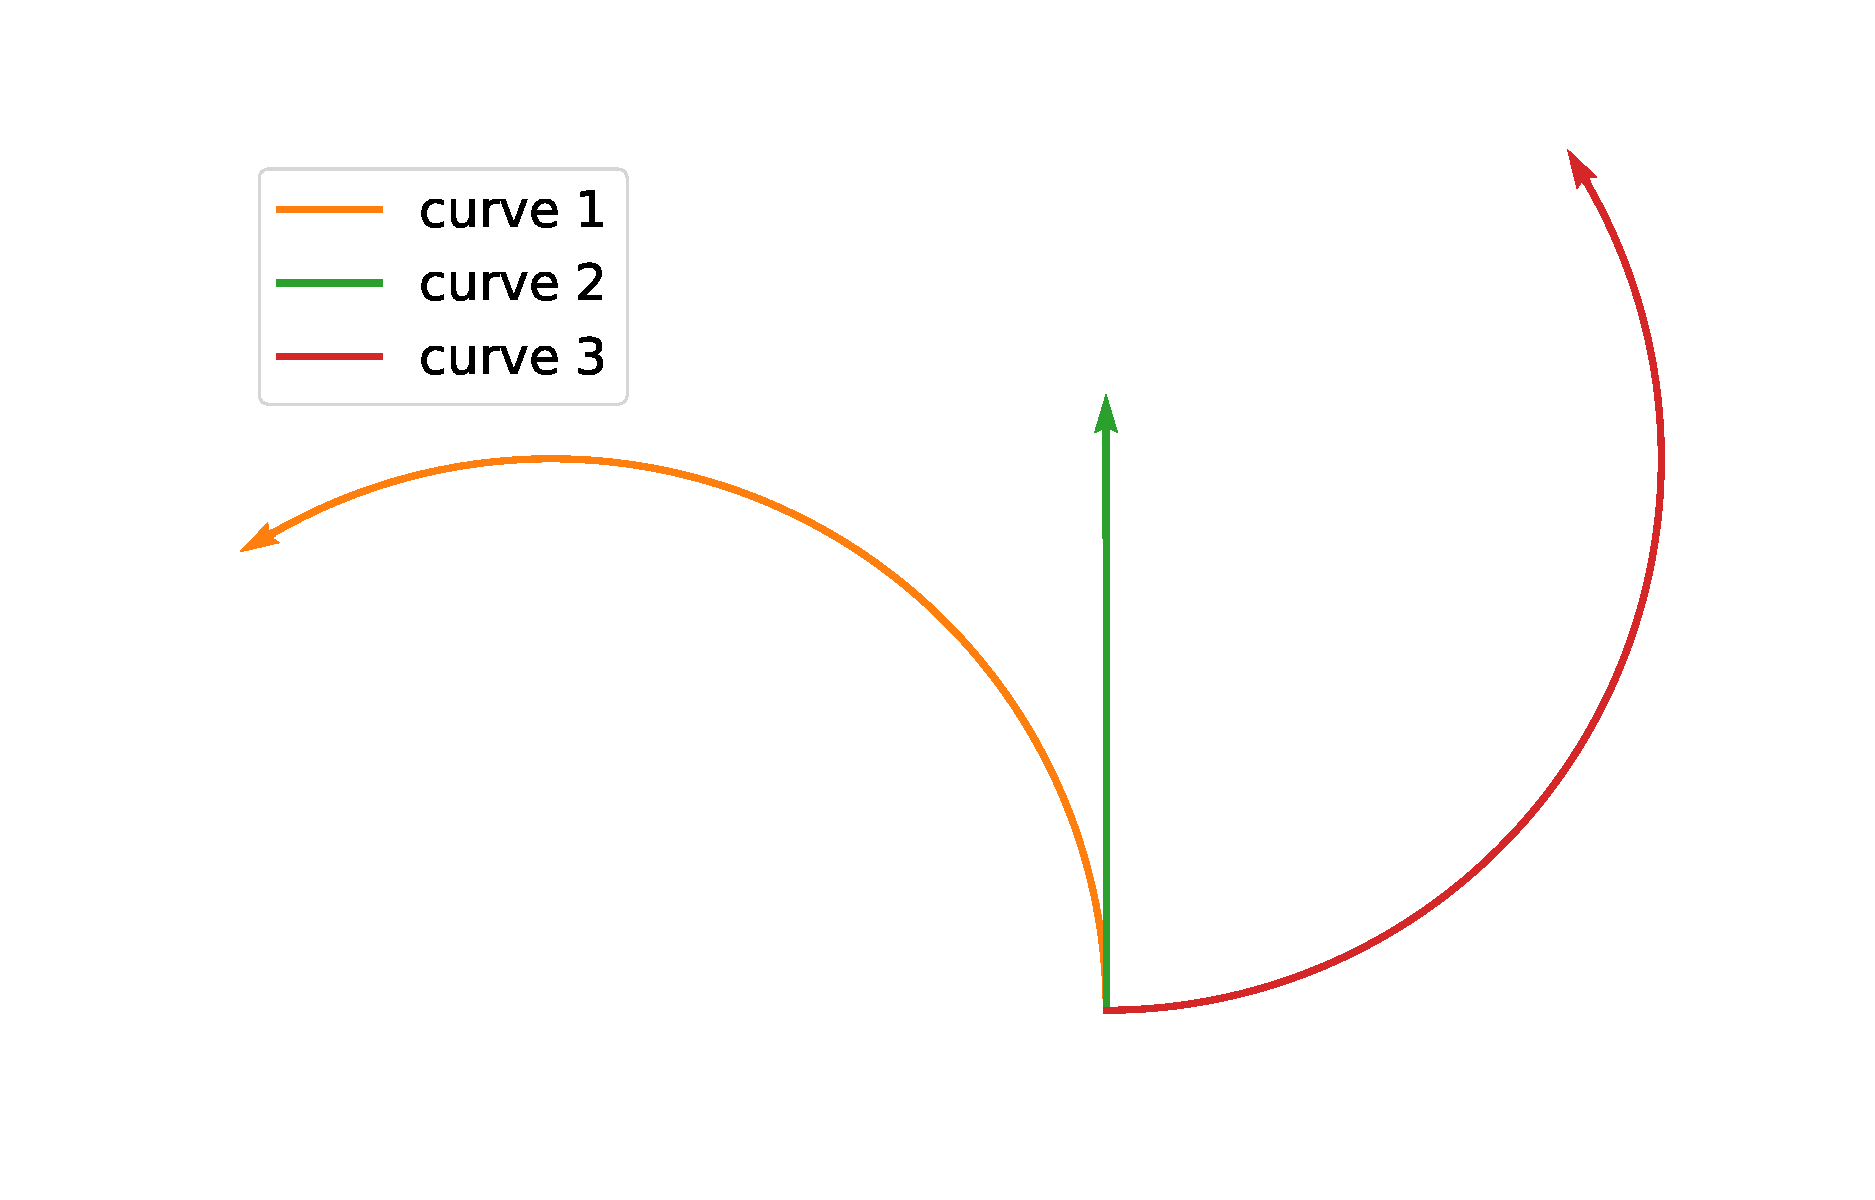
\includegraphics[width=0.45\textwidth]{example_curves.pdf}
\caption{Arc trajectories with different $v$, $\omega$ and $\varphi$. Curve 1 has $v=0.5$, $\omega = 30^\circ/s$ and $\varphi = 90^\circ$. Curve 2 has $v=0.25$, $\omega = 0$ and $\varphi = 90^\circ$.
Curve 3 shares the same $v$ and $\omega$ with curve 1 but having $\varphi = 0$.
All the curves are generated after 4 seconds of movement.
}
\label{arcs}
\end{figure}

To implement arc-based representation, we will need to get the three parameters $v$, $\omega$ and $\varphi$ from the trajectory. 
During the execution of each policy, we record the $x$ and $y$ positions of the robot as well as the time.
For a perfect arc, the points on the trajectory should obey the following equation:
\begin{equation}
(x - A)^2 + (y - B)^2 = A^2 + B^2
\label{circle_equation}
\end{equation}
Where $A$ and $B$ are the $x$ and $y$ coordinates of the center. In Eq. (\ref{circle_equation}) we have forced the curve to pass through the origin, which is the initial position of the robot.
Analytical estimate of the center can be provided by the classical circle fitting method called Kasa method \cite{Kasa_method}.
But this estimation is biased unless the points are symmetrically distributed across the entire circumference \cite{circle_fitting}.
While in most cases, the trajectory of the robot covers less than a quarter circle, and sometimes it is even a straight line.
Hence the Kasa method is not appropriate, and we aim to minimize the unbiased loss function: 
\begin{equation}
\mathcal{L} = 
\sum_{i=1}^N \left[
\sqrt{(x_i - A)^2 + (y_i - B)^2} - \sqrt{A^2 + B^2}
\right]^2
\label{circle_error}
\end{equation}
The optimal solution of this loss function is hard to obtain analytically, hence we use L-BFGS-B \cite{L-BFGS-B} optimization algorithm instead.
After finding the $A$ and $B$, we then get the angular change between each time step.
This is achieved by taking the cross product between the neighbouring points:
\begin{equation}
\begin{gathered}
\sin(\theta_2 - \theta_1) = \\
\frac{(x_1 - A)(y_2 - B)-(y_1 - B)(x_2 - A)}{
\sqrt{(x_1 - A)^2 + (y_1 - B)^2} \sqrt{(x_2 - A)^2 + (y_2 - B)^2}
}
\end{gathered}
\label{delta_theta}
\end{equation}
Because the $\sin (x)$ function is monotonically increasing between $[-\frac{\pi}{2}, \frac{\pi}{2}]$, we can determine the sign of the angular difference (positive for anti-clockwise).
Then, all three parameters can be calculated:
\begin{equation}
\begin{gathered}
\omega = \frac{
\sum_{i=1}^{N-1} \Delta \theta_i \Delta t_i}{
\sum_{i=1}^{N-1} \Delta t_i^2}
\text{ , }
v = \sqrt{A^2 \omega^2 + B^2 \omega^2}
\\
\text{and \,}
\varphi = \operatorname{atan2}(-B, -A) + 
\begin{cases} 
\frac{\pi}{2} & \text{if } \omega > 0 \\
-\frac{\pi}{2} & \text{if } \omega < 0 
\end{cases}
\end{gathered}
\label{all_three_parameters}
\end{equation}
%
To correctly determine the direction, Eq. (\ref{all_three_parameters}) suggests that we need to make sure the $\omega$ is never zero even for a straight line.
In practice, we can achieve this by giving an upper bound to the absolute values of the center coordinates $A$ and $B$, which is the reason we use L-BFGS-B optimization algorithm.
This ensures that the center will not tend to infinity, and hence the absolute value of $\omega$ will always be positive for any trajectory. 
In the extreme case where the robot remains stationary, we must still assign a non-zero value to the $\omega$ to avoid zero division in further calculations, but the direction $\varphi$ can take any value.


One thing to notice is that while the measurement of tangential speed $v$ is always accurate, the measurement of $\omega$ and $\varphi$ can be very noisy in some cases.
For example, if the robot barely moves, the trajectory will be dominated by noise.
Hence the angular velocity $\omega$ and the direction $\varphi$ will become very noisy although they barely make any difference.
While in the case when the robot is travelling fast, $\omega$ and $\varphi$ will be very important and will have accurate measurements as well.
Hence, when modelling the arc-based dynamics representation with GP, it is reasonable to give different noises for different parameters in different trajectories.


To achieve this, we know that the robot coordinates can be regarded as a superposition of the ground truth and a random noise.
Our parameters calculated using Eq. (\ref{all_three_parameters}) correspond to the best-fit arc, and are also affected by this noise.
If we only focus on the final position after executing a policy, and we assume that the random noise only depends on the environment but not the policies, we can write:
%
\begin{equation}
\begin{gathered}
\sigma_{\hat{x}}^2 + \sigma_{\hat{y}}^2 = 2 \sigma_{\epsilon}^2
\end{gathered}
\label{summed_variance}
\end{equation}
%
where we have assumed the same noise variance $\sigma_{\epsilon}^2$ on both $x$ and $y$ axis.
The $\hat{x}$ and $\hat{y}$ denote the final coordinates given by the arc, where:
\begin{equation}
\begin{gathered}
\hat{x}(t | v, \omega, \varphi) 
%= \int_0^t v \cdot \cos(\varphi + \omega \tau) d\tau 
= \frac{v}{w} \left[ \sin(\omega t + \varphi) - \sin(\varphi) \right]
\\
\hat{y}(t | v, \omega, \varphi) 
%= \int_0^t v \cdot \sin(\varphi + \omega \tau) d\tau 
= \frac{v}{w} \left[ \cos(\varphi) - \cos(\omega t + \varphi) \right]
\end{gathered}
\label{position_from_arc}
\end{equation}
%
The term $\sigma_{\hat{x}}^2$ and $\sigma_{\hat{y}}^2$ in Eq. (\ref{summed_variance}) are related to the uncertainties in our measurement of $v$, $\omega$ and $\varphi$.
To study this relation, we model the error propagation with linear approximation, where the error of the random variable $f(x, y, z)$ is given by \cite{error_analysis}:
\begin{equation}
\begin{gathered}
\sigma_f^2 \approx
\frac{\partial f}{\partial x}^2 \sigma_x^2
+ \frac{\partial f}{\partial y}^2 \sigma_y^2
+ \frac{\partial f}{\partial z}^2 \sigma_z^2
\end{gathered}
\label{error_prapagation}
\end{equation}
Eq. (\ref{error_prapagation}) requires the random variables $x$, $y$ and $z$ be independent, which is consistent with our design.
Combining the above three equations, we will get:
\begin{equation}
\begin{gathered}
2\sigma_{\epsilon}^2 \approx 
\left(
 \frac{\partial \hat{x}}{\partial v}^2
 + \frac{\partial \hat{y}}{\partial v}^2
\right) \sigma_v^2 
\\ +
\left(
\frac{\partial \hat{x}}{\partial \omega}^2
+
\frac{\partial \hat{y}}{\partial \omega}^2
\right) \sigma_{\omega}^2 
 +
\left(
\frac{\partial \hat{x}}{\partial \varphi}^2
+ 
\frac{\partial \hat{y}}{\partial \varphi}^2
\right) \sigma_{\varphi}^2
\end{gathered}
\label{combined_error_relation}
\end{equation}
Since the LHS of the Eq. (\ref{combined_error_relation}) is invariant to the policies, it is reasonable to assume that:
\begin{equation}
\begin{gathered}
\sigma_v^2 \propto
\frac{1}{
\frac{\partial \hat{x}}{\partial v}^2 
+ \frac{\partial \hat{y}}{\partial v}^2 + \varepsilon_v}
\\
\sigma_{\omega}^2 \propto
\frac{1}{
\frac{\partial \hat{x}}{\partial \omega}^2
+
\frac{\partial \hat{y}}{\partial \omega}^2 + \varepsilon_{\omega}} 
\\
\sigma_{\varphi}^2 \propto
\frac{1}{
\frac{\partial \hat{x}}{\partial \varphi}^2
+ 
\frac{\partial \hat{y}}{\partial \varphi}^2 + \varepsilon_{\varphi}} 
\end{gathered}
\label{noises_for_v_w_phi}
\end{equation}
where a positive small constant is added at the each denominator for numerical stability.
This result is very reasonable as higher dependency on the parameter leads to smaller noise.
Although Eq. (\ref{noises_for_v_w_phi}) doesn't give the exact value for the noises, it provides a method to calculate relative noises between different policies in the same environment.



\subsection{Clustering the Dynamics with Dirichlet Processes}
So far, we have determined the basis for our linear prior mean function, the input space, different representations of dynamics as well as the way to calculate relative noises.
To cluster the historical data with DP, we still need the prior distribution $H$ for the detailed parameters. 
In our case where the dynamics are modelled by GP, these parameters include the weights $\bm{w}$ for the linear mean function, the length scales $\bm{l}$ and the prior variance $\alpha_0$ for the kernel, and the noises $\sigma_{n}^2$ for covariance matrix.


This is hard to do since we have little knowledge.
Even if we could give a perfect prior distribution, the integrals in Eq. (\ref{integral_1}) and Eq. (\ref{integral_2}) are intractable.
The solution is use Monte Carlo sampling in simulation combined with a trick called posterior convergence estimate.
We can see that these parameters are all related to the environment.
The Monte Carlo sampling is to collect a sample of these environment-related parameters from the simulation as our prior distribution $H$.
To do this, we first randomize the simulation settings to get a sample of simulated environments.
We then collect a sufficient amount (e.g. 64) of interaction data from each environment and find the detailed parameters using maximum likelihood estimate (MLE):
\begin{equation}
\bm{\theta}^* = 
\arg \max_{\bm{\theta}} \, p(\bm{y}|\bm{\theta})
= \arg \min_{\bm{\theta}} \, -\log p(\bm{y}|\bm{\theta})
\label{MLE}
\end{equation}
The Monte Carlo sampling seems computationally expensive. But note that the sample amount for each environment is small and invariant to the size of the repertoire.
Hence it is much cheaper to do than finding the basis for the prior mean function, where we need to evaluate all the policies in several environments.


The probabilistic model in our case is a product of GPs over the dimensions, and $p(\bm{y}|\bm{\theta})$ can be calculated from Eq. (\ref{multi_normal}):
\begin{equation}
\begin{gathered}
-\log p(\bm{y}|\bm{\theta}) = \sum_{d} -\log p(\bm{x}_{d}|\bm{\theta}_d)
\\
= \frac{1}{2} \sum_{d}
(\bm{x}_{ d} - \bm{\mu}_{\bm{\theta}_d})^T \bm{\Sigma^{-1}}_{\bm{\theta}_d} (\bm{x}_{d} - \bm{\mu}_{\bm{\theta}_d})
\\ + \sum_{ d} \left[ \frac{N}{2}\log(2\pi) 
+ \log \det(\bm{\Sigma}_{ \bm{\theta}_d}) \right]
\end{gathered}
\label{nll}
\end{equation}
where the weights $\bm{w}_d$ are encoded in $\bm{\mu}_{\bm{\theta}_d}$, and the rest of the parameters are encoded in $\bm{\Sigma}_{\bm{\theta}_d}$.
It is worth noting that the noise $\sigma_n^2$ in displacement-based representation is the same for all policies; while in arc-based representation, Eq. (\ref{covariance_matrix}) needs to be modified:
\begin{equation}
\bm{\Sigma} = \bm{K}(\bm{x_{1:N}}, \bm{x_{1:N}}) + \sigma_{n}^2 \bm{D}
\label{modified_covariance_matrix}
\end{equation}
where matrix $\bm{D}$ is a diagonalized matrix with entries calculated according to Eq. (\ref{noises_for_v_w_phi}).
The optimal solution of Eq. (\ref{MLE}) can be obtained using optimization algorithms like L-BFGS-B. The integrals in Eq. (\ref{integral_2}) and Eq. (\ref{integral_1}) hence become the averages of finite number of terms:
\begin{equation}
\begin{gathered}
p(y_i|c_i, \bm{y}_{-i}, \bm{c}_{-i}) = 
\sum_{l=1}^L p(y_i|\bm{\theta}^{(l)})
p(\bm{\theta}^{(l)}|c_i, \bm{y}_{-i}, \bm{c}_{-i})
\\
p(y_i|c_i \neq j \, \text{for any} \, n_j \neq 0) = 
\frac{1}{L} \sum_{l=1}^L p(y_i|\bm{\theta}^{(l)})
\end{gathered}
\label{MC_prior_integral}
\end{equation}
Where the posterior distribution is:
\begin{equation}
p(\bm{\theta}^{(j)}|c_i, \bm{y}_{-i}, \bm{c}_{-i}) = 
\frac{
\prod_{c_k=c_i, k \neq i} p(y_k|\bm{\theta}^{(j)})}
{\sum_{l=1}^L \prod_{c_k=c_i, k \neq i} p(y_k|\bm{\theta}^{(l)})}
\label{MC_posterior}
\end{equation}
In practice, it is much easier and numerically stable to work with logarithm likelihoods as in Eq. (\ref{nll}), as the direct product of likelihoods will very likely lead to overflow.


Although the integrals are now made tractable, this method has two fatal shortages.
First, the Monte Carlo sampling only provides limited precision of the parameters.
As each cluster grow larger, Eq. (\ref{MC_posterior}) implies that the set of parameters that is closest to the ground truth will eventually make up 100\% of the posterior weight.
Hence, the number of clusters will not exceed the amount of sampled priors. 
Second and more importantly, the prior collection is made in simulation, which ensures no extrapolation to the real-world.
To solve these two shortages, we introduce a trick called posterior convergence estimate.
As a cluster gathers more data, the posterior distribution of its parameters will become narrower and more centred closer to the ground truth (see Fig \ref{posterior_convergence}).
\begin{figure}[h]
\centering
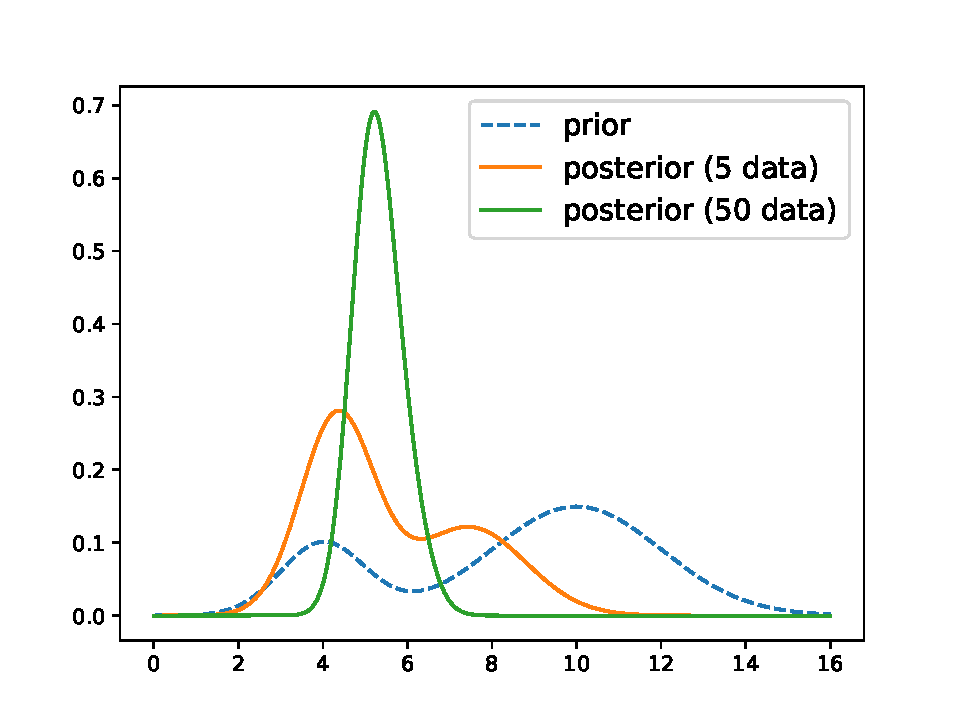
\includegraphics[width=0.45\textwidth]{posterior_convergence.pdf}
\caption{Example of the convergence of parameter posterior in DPMM.
Data are sampled from a infinite mixture of Gaussians, where the variance is fixed at 4, and the mean is given by a Gaussian mixture as the prior.
As the cluster grows larger, the posterior of the mean becomes more narrowed and centred at the ground truth (5.5).
}
\label{posterior_convergence}
\end{figure}
%
When the cluster size is large, we can safely assume that the posterior becomes a sharp spike.
Hence, we may treat it as a Dirac delta distribution, and Eq. (\ref{integral_1}) becomes:
\begin{equation}
\begin{gathered}
p(y_i|c_i, \bm{y}_{-i}, \bm{c}_{-i}) \approx 
\int p(y_i|\bm{\theta})
\delta (\bm{\theta} - \bm{\theta}^*)
d\bm{\theta}
\\
= p(y_i|\bm{\theta}^*)
\end{gathered}
\label{posterior_convergence_estimate}
\end{equation}
This is called posterior convergence estimate, and the center of this Dirac delta is located using MAP. 
This means we refit the parameters for large clusters (with data size above a threshold, e.g. 30) as their posterior.
This design is to leverage the fact that for small clusters the posteriors haven't converged, and their integration can be efficiently approximated by Eq. (\ref{MC_prior_integral}).
While for large clusters, their posterior cannot be efficiently represented by any prior, so we allow them to determine the best parameters based on their data.
The only thing that such prior should satisfy is that it covers a variety of possible cases.
Thus, the use of Monte Carlo sampling for the prior acts like a guide for smaller clusters, and neither the coverage of parameters or the number of clusters is constrained by the prior. 


Because we have no access to the analytical form of the prior to do MAP, we can use MLE instead (for large data size, MLE and MAP gives similar results).
Hence, during Gibbs sampling, the likelihood of an episode belonging to a large cluster is calculated according to Eq. (\ref{posterior_convergence_estimate}), while the likelihood of belonging to a small cluster is calculated using the first equation in Eq. (\ref{MC_prior_integral}).
As mentioned previously, the episode needs to be removed from its current cluster which will affect the posterior when calculating the likelihood of this episode staying in its current cluster.
For small cluster, we can recalculate the posterior using Eq. (\ref{MC_posterior}).
For large cluster, this means the parameter $\bm{\theta}^*$ needs to refitted with this episode removed, if the data size is still large enough without this episode. 
After each resample step, we also need to refit the parameters for large clusters if any change is made.
Be aware that the subscript $i$ in Eq. (\ref{MC_prior_integral}), Eq. (\ref{MC_posterior}) and Eq. (\ref{posterior_convergence_estimate}) refers to each episode instead of each individual interaction data. 
Similarly, the $n$ in Eq. (\ref{indicator_posterior_3}) corresponds to the number of episodes instead of the amount of data.


In practice, refitting all the parameters in each step of Gibbs sampling could lead to performance issues as the Gibbs sampling cannot be paralleled.
It is much cheaper to just refit the weights for the prior mean function and leave the rest of the parameters fixed.
It is reasonable as the prior is most important and can be obtained analytically:
\begin{equation}
\bm{w}_d^* = \left(\sum_{i=1}^n
\bm{X}_i^T \bm{\Sigma}_{i, \bm{\theta}_d}^{-1} \bm{X}_i
\right)^{-1} \sum_{i=1}^n \bm{X}^T_i \bm{\Sigma}_{i, \bm{\theta}_d}^{-1} \Delta \bm{x}_{i, d}
\label{refitted_weights}
\end{equation}
where the summation is made over all the episodes in the cluster.
$\Delta \bm{x}_{i, d}$ is the real-world distortions of the $i^{\text{th}}$ episode.
$\bm{X}_i$ is the coordinate matrix of this episode, where each row gives the coordinates of the policy corresponding to each interaction.
Since the rest of the parameters are fixed, the covariance matrix $\bm{\Sigma}_{i, \bm{\theta}_d}$ is generated using the most likely prior sample.



\subsection{Learning the Dynamics Online}
After having clustered the historical data, we can use the result to assist adaptation.
In RTE, we learn the distortion online using GPs, where the parameters (prior mean function, kernel etc.) are determined manually.
In our method, the dynamics is modelled with an infinite mixture of GPs. 
The GP parameters are given by the posterior distribution found with historical data, which is a mixture model of finite terms:
\begin{equation}
p(\bm{\theta}) = \sum_j \frac{n_j}{n + \alpha} p(\bm{\theta}|c=j) 
+ \frac{\alpha}{n + \alpha} H(\bm{\theta})
\label{trained_mixture_model}
\end{equation}
where the summation is made over the clusters containing at least one episode, and $p(\bm{\theta}|c=j)$ denotes the posterior for the $j^{\text{th}}$ cluster.
Each instance of $\bm{\theta}$ sampled from $p(\bm{\theta})$ is a certain configuration of parameters of GP.
The last term results from the important property of DPMM that there is always a non-zero probability that we will get a new cluster (face a new situation).
The online learned distortion is integrated over the posterior of $\bm{\theta}$ conditioned on the collected real-world interactions:
\begin{equation}
\begin{gathered}
p(x^*_d|\bm{x}_{1:N}) 
\\
= \sum_j p(c=j| \bm{x}_{1:N}) \int p(x^*_d|\bm{\theta}, \bm{x}_{1:N})p(\bm{\theta}|c=j, \bm{x}_{1:N}) d\bm{\theta} 
\\
+ p(c \neq j, \forall j|\bm{x}_{1:N}) \int p(x^*_d|\bm{\theta}, \bm{x}_{1:N}) p(\bm{\theta} | \bm{x}_{1:N}) d\bm{\theta}
\end{gathered}
\label{MGP_posterior}
\end{equation}
where the indicator probability is given by:
\begin{equation}
\begin{gathered}
p(c=j| \bm{x}_{1:N}) 
= \frac{n_j \cdot p(\bm{x}_{1:N}|c=j)
}{Z}
\\ 
p(c \neq j, \forall j| \bm{x}_{1:N})
= \frac{\alpha \cdot p(\bm{x}_{1:N}|c \neq j, \forall j)
}{Z}
\end{gathered}
\label{MGP_indicator}
\end{equation}
where $\bm{x}_{1:N}$ stands for the collected ($N$ number of) interaction data during deployment.
This is complicated and requires calculating multiple integrals over the posteriors. 
Fortunately, if we have applied posterior convergence estimate for $p(\bm{\theta}|c=j)$, we will have:
\begin{equation}
\begin{gathered}
\int p(x^*_d|\bm{\theta}, \bm{x}_{1:N})p(\bm{\theta}|c=j, \bm{x}_{1:N}) d\bm{\theta} \approx p(x^*_d|\bm{\theta}^*_j, \bm{x}_{1:N})
\\
\text{and } p(\bm{x}_{1:N}|c=j) \approx p(\bm{x}_{1:N}|\bm{\theta}^*_j)
\end{gathered}
\label{posterior_convergence_simplification}
\end{equation}
where $\bm{\theta}^*_j$ denotes the optimal parameters for the cluster $j$.
In actual implementation, the clustering of historical data with DP is conducted in the archive management system where expensive data processing is available. 
The results are saved as an adaptation system to be used (downloaded) by individual robots.
The adaptation system is independent from the archive, and we are free to make simplifications for embedded systems.
Hence, we can apply posterior convergence estimate for all the clusters we have found for simplicity.
For clusters that are not large enough to refit the parameters, we will just use the parameters of the most likely prior sample.
This might be inappropriate for clusters that are very small, and hence we can discard them from the adaptation system.


We still need to solve the two integrals in Eq. (\ref{MGP_posterior}) and Eq. (\ref{MGP_indicator}) for the case of a new cluster.
This can be hard even with the Monte Carlo sampling. 
If our MC prior does not cover this new situation, our method could fail.
In this paper, we take a very simple solution by using RTE to incorporate this new situation.
Although RTE is not optimized for any environment, it offers a satisfying baseline performance in all situations.
The non-zero probability of encountering new cases secured by DP and the use of RTE ensures that we can always adapt well to new situations and hence will never over-fit to the training data.
Combined with Eq. (\ref{posterior_convergence_simplification}), the distortion becomes:
\begin{equation}
\begin{gathered}
p(x^*_d|\bm{x}_{1:N}) 
= \sum_j p(c=j| \bm{x}_{1:N}) p(x^*_d|\bm{\theta}^*_j, \bm{x}_{1:N})
\\
+ \,\, p(c \neq j, \forall j|\bm{x}_{1:N})  p(x^*_d|\bm{x}_{1:N}, \text{RTE})
\end{gathered}
\label{simplified_distortion}
\end{equation}
where the indicator probabilities are:
\begin{equation}
\begin{gathered}
p(c=j| \bm{x}_{1:N}) 
= \frac{n_j \cdot p(\bm{x}_{1:N}|\bm{\theta}^*_j)
}{Z}
\\ 
p(c \neq j, \forall j| \bm{x}_{1:N})
= \frac{\alpha \cdot p(\bm{x}_{1:N}|\text{RTE})
}{Z}
\\ \text{where }
Z = \sum_k n_k \cdot p(\bm{x}_{1:N}|\bm{\theta}^*_k) + \alpha \cdot p(\bm{x}_{1:N}|\text{RTE})
\end{gathered}
\label{simplified_indicator}
\end{equation}
In contrast to RTE, our online learning of the dynamics consists of two levels.
The first level is to use the real-world data to figure out the situation that the robot is in, which is the indicator probability given by Eq. (\ref{simplified_indicator}).
Considering the dynamics can be distinct for different environments, the robot should be able to quickly figure out its current situation.
Since each situation has a prior mean function that can give estimation of the dynamics without further data, our method should be able to provide fast online learning of the real-world dynamics with much higher data-efficiency than RTE.
The second level is to learn the residual dynamics, which is the part of the distortion failed to be captured by the prior mean, using the kernels optimized for each situation.
The final prediction of dynamics given by Eq. (\ref{simplified_distortion}) is a mixture of Gaussians.
Where each mixture component has mean and variance calculated using Eq. (\ref{GP_posterior}), and the mixture weights are equal to the probabilities of being in each situation.
This learned dynamics can then be used by the robot to correct its motion accordingly.